In this chapter the product and its requirements are described in order to provide a background for the "Requirements specification" part and make it easier to understand.

\section{Product perspective}
% Here we put the application into perspective with other related products, interfaces/communication means should be identified
\subsection{User interfaces} % aka "Ease of use"
\label{subsec:user_interfaces}
The user should be able to interact with the system in three ways:
\begin{itemize}
	\item{Web application}: is strongly cross-platform and then accessible from any device that can browse the web
	\item{Mobile application}: accessible from smartphones and mobile devices in order to guarantee portability and ease of use
	\item{On-Board computer}: accessible from the inside of any PowerEnjoy car, it must be extremely straightforward and let the user focus on the actual interaction
\end{itemize}
A common and friendly UI should be provided to create a sort of logical connection between the three different applications and make the user feel comfortable.

\subsection{Hardware interfaces}
The web application has no other hardware constraints despite the ones specified in subsection \ref{subsec: hw_constraints}, it should run on any device meeting such minimum requirements. Mobile application has to communicate with GPS, Antenna and WiFi modules in order to retrieve location and query the server, requirements easily met by any modern smartphone.
\\On-Board computers require a car with self-diagnostic and reporting capability.
\subsection{Software interfaces}
The web application should support devices running any modern browser while the mobile application will be developed and supported on iOS, Android and eventually WP. 
\\On-Board computer's application is device-specific and will then be designed based on the ad-hoc hardware, embedded OS and APIs.
\section{Product functions}
The system that we are to develop must let users register and then login in order to manage their account and actively access the service. The provided functionalities are clearly enumerated in section \ref{sec: proj_objectives} and here graphically described to ease the complete comprehension of the system.

\begin{figure}[!ht]
	\centering
	\vspace{0.2cm}
	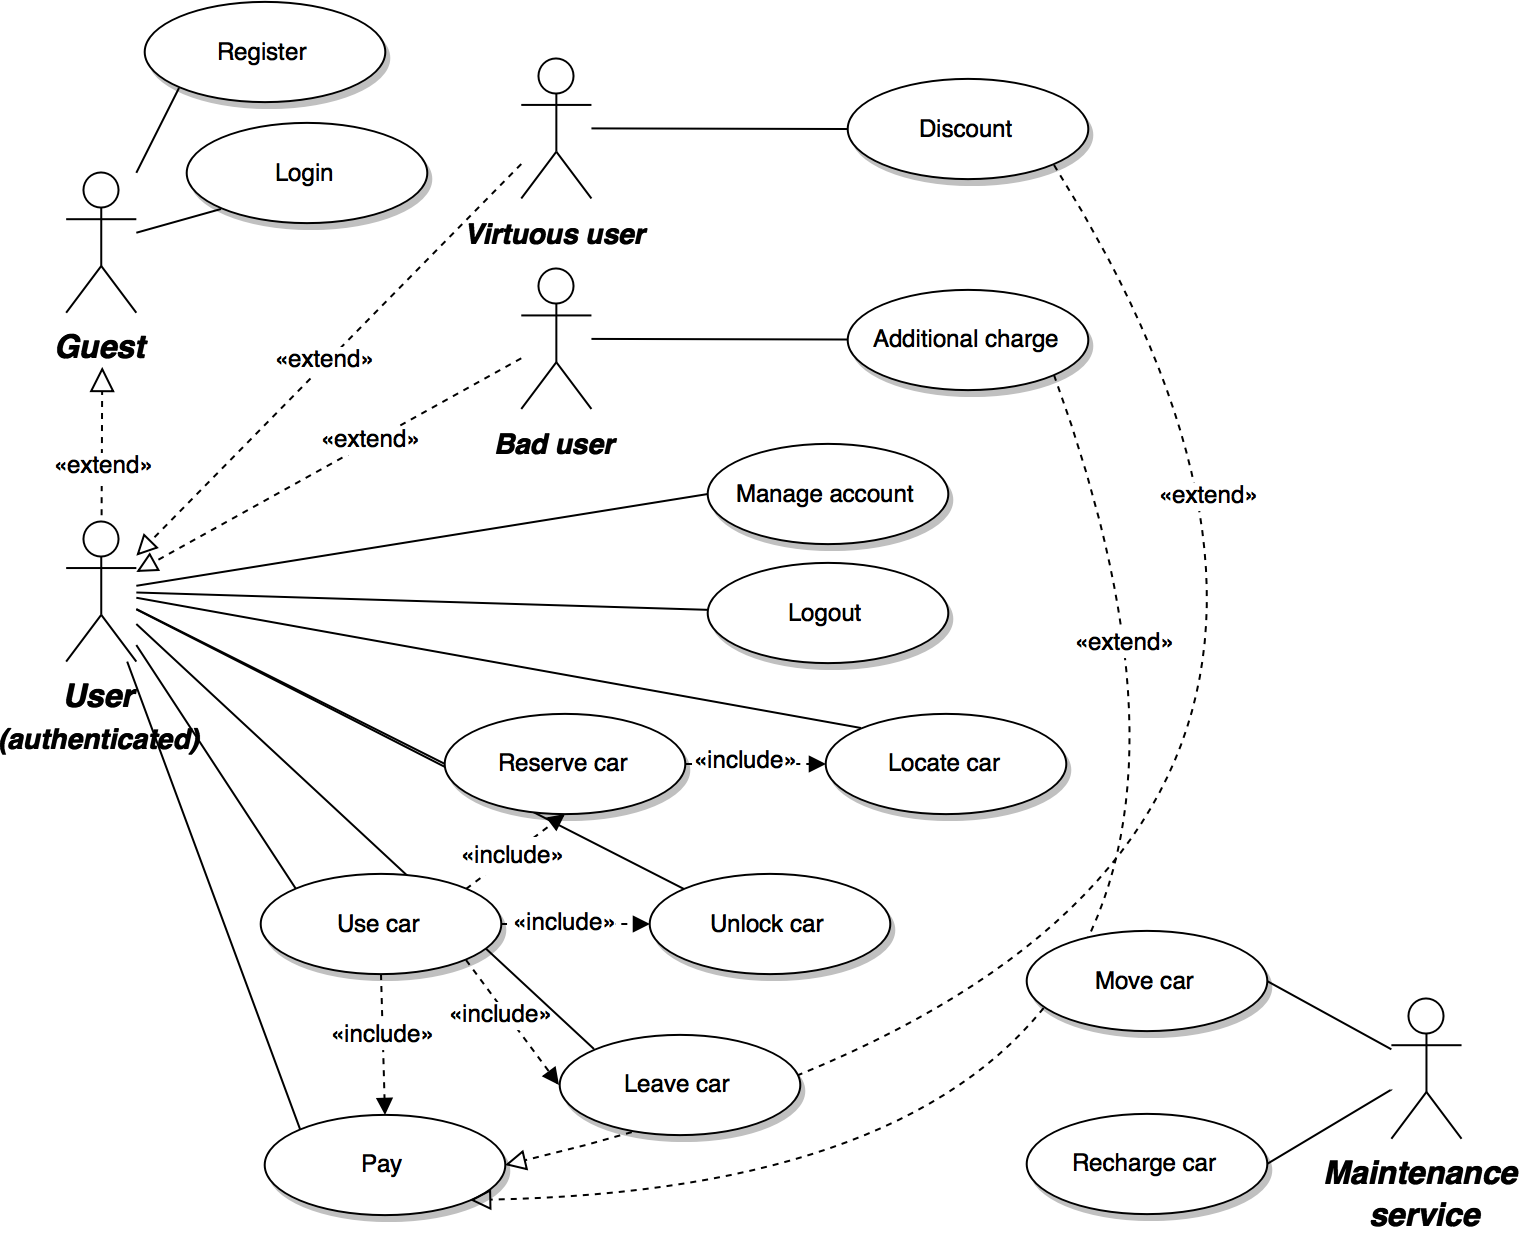
\includegraphics[width=1.0\textwidth]{/RASD/main_use_case}\\ 
	\vspace{0.5cm}
	\caption{Main use-case representing all the functionalities of the system} \label{fig:main_use_case} 
\end{figure}

\section{User characteristics}
The application should target users with a valid driving license, being at least 18 and providing a secure payment method, which must be checked before any reservation.
\\Additional legal requirements might be necessary, especially if the service is intended to spread into foreign countries
\section{Constraints}
\subsection{Regulatory policies}
Users must allow the system to collect and use personal data according to a privacy policy: data such as personal details, payment methods, transactions and locations are stored and processed in order to provide a higher service quality.
\subsection{Hardware limitations}
\label{subsec: hw_constraints}
Hardware requirements are extremely different depending on the application that is being considered; in this document, though, the on-board computer's hardware won't be discussed.
The web application development demand two main hardware constraints: 
\begin{itemize}
	\item{Stable internet connection}
	\item{Modern(supported) web browser}
\end{itemize}
The mobile application will be deployed for mobile devices, so even the memory constraints are consistents:
\begin{itemize}
	\item{ARM architecture}
	\item{At least 1GB of RAM}
	\item{At least 50MB of available storage}
	\item{Up-to-date operating system (minimum API level or OS version)} 
	\item{Stable internet connection}
	\item{GPS module may be useful but not necessary to access the service}
\end{itemize}
\subsection{Parallel operation}
The system must support heavy parallel processing because of the high number of users that are to access the service potentially at the same time.
\subsection{Reliability requirements}
The system must be opportunely reliable in order to support users while accessing the service, a 3-nines availability (\textasciitilde9hours/year) is more than enough for a non life-critical system 
\subsection{Safety and security considerations}
% todo: identify safety considerations(driving licence, safe areas, fraud, user/car damage...)
Lorem ipsum dolor sit amet, consectetur adipiscing elit, sed do eiusmod tem- por incididunt ut labore et dolore magna aliqua. Ut enim ad minim veniam, quis nostrud exercitation ullamco laboris nisi ut aliquip ex ea commodo conse- quat. Excepteur sint occaecat cupidatat non proident, sunt in culpa qui officia deserunt mollit anim id est laborum.
\section{Assumptions and dependencies}
In order for the system to work properly some domain assumptions are needed:
\begin{itemize}
	\item{Sensors and devices needed to support the functionalities of the system are already installed on vehicles}
	\item{Cars are equipped with a standard diagnostic connector and are using OBD-II communication protocols}
	\item{The GPS signal is sufficiently accurate ($\pm5m$ accuracy with A-GPS)}
	\item{If an User is reserving a car she can't try to find an other car}
\end{itemize}
% todo: complete assumptions listening to recordings and consulting notes on the firs lab